\documentclass[hyperref={bookmarks=false},aspectratio=169]{beamer}
\usepackage[utf8]{inputenc}
\usepackage{tikz}
\usetikzlibrary{arrows.meta}

% ---------------  Define theme and color scheme  -----------------
\usetheme[sidebarleft]{Caltech}  % 3 options: minimal, sidebarleft, sidebarright

% ------------  Information on the title page  --------------------
\title[Florian for Maria Mushtaq]{\Huge{Florian Duzés} \\for \bfseries{Maria Mushtaq}}

\subtitle{A brief interview}

\author[Florian Duzés]{Florian Duzés}


\date[2025]{June 18, 2025}
%------------------------------------------------------------

\AtBeginSection[]
{
  \begin{frame}
    \frametitle{Table of Contents}
    \tableofcontents[currentsection]
  \end{frame}
}

%------------------------------------------------------------

\begin{document}

\begin{frame}
    \titlepage
\end{frame}


%---------   table of contents after title page  ------------
\begin{frame}
\frametitle{Summary}
\tableofcontents
\end{frame}
%---------------------------------------------------------

\section{General presentation}

\begin{frame}{Whoami}

  \begin{columns}
    \begin{column}{0.7\textwidth}
      \begin{block}{Essential}
        \begin{itemize}
          \item<1-> 23 years old
          \item<2-> From Albi, South of France
          \item<3-> Languages :
          \begin{itemize}
            \item<3-> French, Spanish, English
          \end{itemize}
          \item<4-> Hobbies
          \begin{itemize}
            \item<4-> Sport
            \item<4-> Gastronomy
            \item<4-> Reading
            \item<4-> Cinema
          \end{itemize}
          \item<5-> Lot of Benevolent work in youth animation
        \end{itemize}
      \end{block}
    \end{column}

    \begin{column}{0.3\textwidth}
      \framebox[1\width]{
\includegraphics[scale = 0.15]{./img/me/me.jpeg}}
      \onslide<2->{\framebox[1\width]{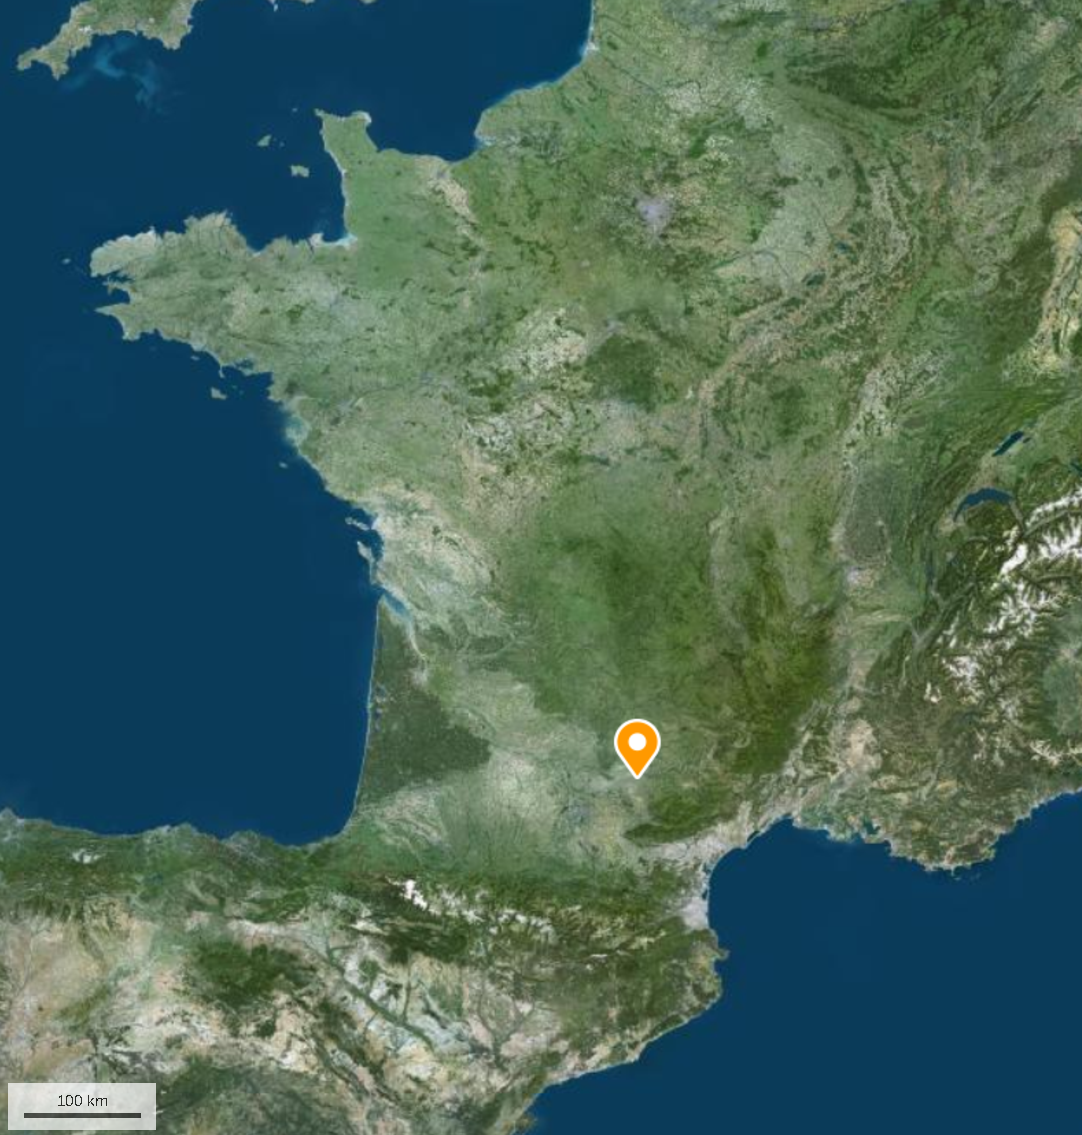
\includegraphics[scale = 0.2]{./img/me/map.pdf}}    }
    \end{column}
  \end{columns}
  
\end{frame}

\section{Academic background}

\begin{frame}{Evolution \& Changes}
  \begin{alertblock}{Bachelor}
    \begin{itemize}
      \item[1st y] Bachelor in mathematics
      \item[1/2 y] Dual Bachelor in Mathematics and Computer Science
      \item[3rd y] Bachelor's degree in Computer Science
      \begin{itemize}
        \item Specialisation AI
      \end{itemize}
    \end{itemize}
  \end{alertblock}
    \begin{tikzpicture}[overlay]
      \node (img) at (10,-1)  {
\includegraphics[scale=0.19]{img/logo/LOGO_CHAMPOLLION.png}};
  \end{tikzpicture}

\end{frame}


\begin{frame}{Higher studies}
\begin{alertblock}{Master}
  \begin{itemize}
    \item 1st year
    \begin{itemize}
      \item Cryptography principles
      \begin{itemize}
        \item number theory, abstract algebra, and probability theory...
      \end{itemize}
      \item Computer Security
      \begin{itemize}
        \item Network security, Software Security, Programming
      \end{itemize} 
    \end{itemize}
  \end{itemize}

  \begin{itemize}
    \item 2nd year - only options
    \begin{itemize}
      \item Cryptanalysis
      \item Post Quantum Cryptography
      \item Chip security
      \item OS Security
      \item PQ algorithmic
    \end{itemize}
  \end{itemize}
  \begin{tikzpicture}[overlay]
      \node (img) at (10,1)  {
\includegraphics[scale=0.12]{img/logo/logo-univ-bordeaux.png}};
  \end{tikzpicture}
\end{alertblock}
\end{frame}

\section{Projects and internship}

\begin{frame}{Achievements}
  \begin{block}{Temporal Order}
    \begin{itemize}
      \item<1-> Chat in local Network, C
      \item<2-> C compiler, Ocaml
      \item<3-> HE Chat - Paillier cryptosystem, C
      \item<4-> PRNG introduction, research article
      \item<5-> ECDSA side channels attacks, Sagemath  
    \end{itemize}
  \end{block}
\end{frame}

\begin{frame}{Inria internship}
  \begin{block}{Binsec \& HACL*}
    \begin{itemize}
      \item Automation
      \item CT detection
      \item Compiler diversity
      \begin{itemize}
        \item x86, arm, riscV
      \end{itemize}
    \end{itemize}
  \end{block}
\end{frame}

\section{Future projections}

% secure & Safe Hardware
\begin{frame}{SSH lab}
  
  \begin{block}{How do I see myself working with SSH Lab}
    \begin{itemize}
      \item INRIA Internship
      \pause
      \item General Set-Up
      \item Installing Gem5
      \item Tutorials \& reading articles
      \item Dive into subjects / seminairs / presentation
    \end{itemize}
  \end{block}
\end{frame}

\begin{frame}{In my mind}
  \begin{block}{Imagination}
    \begin{itemize}
      \item SCA / CPA / CT attacks
      \item Automatisation
      \item RiscV transfer of knowledge
    \end{itemize}
  \end{block}
\end{frame}

\begin{frame}{Offers - interships references}
  
  \begin{block}{Preferences}
    \begin{enumerate}
      \item Modeling \& Formalising timing based SC
      \item Dev framework for RL (with RTL simul + board exec)
    \end{enumerate}
  \end{block}
\end{frame}


\begin{frame}
  \begin{center}
    \Huge 
    \textit{\textcolor{Night_blue}{ Merci.}}\\
    
\includegraphics[scale=0.2]{img/Filet-7pt.png}
  \end{center}
\end{frame}


\begin{frame}{Looking forward}
  
  \begin{block}{Thesis ?}
    \begin{itemize}
      \item Desire \dotfill \textcolor{Green}{I want}
      \item Curiousity\dotfill\textcolor{Green}{Yes}
      \item Open minded\dotfill \textcolor{Green}{Yes}
      \item Can I ? \dotfill \textcolor{Green}{Yes}
    \end{itemize}
    \begin{tikzpicture}
      \draw[-] (-1,0) -- (12.3,0);
    \end{tikzpicture}
    \begin{itemize}
      \item Should I ?\dotfill \textcolor{Green}{YES !}
    \end{itemize}
  \end{block}
\end{frame}




%---------------------------------------------------------


\end{document}